\chapter{Demonstra��o de cria��o de chave e descriptografia com GnuPG}
\label{apend:2}
Como exemplo do acesso ao chaveiro por linha de comando, a seguir teremos o exemplo da gera��o de um novo par de chaves PGP atrav�s do GnuPG e de como us�-la para criptografar o conte�do textual de um arquivo e descriptograf�-lo logo depois.

Para a gera��o de novas chaves, deve-se usar o comando gpg seguido da instru��o --gen-key. A aplica��o ent�o questionar� o usu�rio a respeito dos detalhes da opera��o e, ap�s a conclus�o, uma nova chave privada estar� dispon�vel no chaveiro. Essas informa��es dizem respeito ao tipo de chave desejada, aos dados do usu�rio, como nome e endere�o de e-mail, a validade da chave e a senha que proteger� a chave privada. O ser� informado ao final da cria��o do identificador da sua chave, que no exemplo abaixo � o c�digo A4D9 244A 24DE 2555 3177  C88B ED54 9C38 274F 10C4. O comando gpg --list-keys pode ser usado para listar as chaves conhecidas, revelando a nova chave rec�m-criada.

\begin{figure}[H]
 \centering
 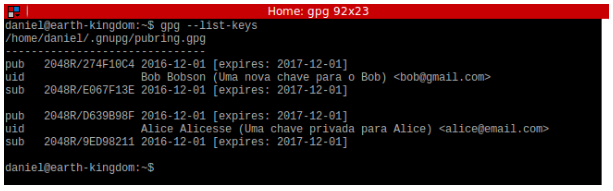
\includegraphics[width=0.9\textwidth]{./fig/2-listar-chaves.png}
 \caption{Listagem de chaves presententes no chaveiro GnuPG}
 \label{fig:exemploFig2}
\end{figure}


Todas os demais par�metros poss�veis podem ser consultados com o comando gpg --help e man gpg. 

\begin{figure}[H]
 \centering
 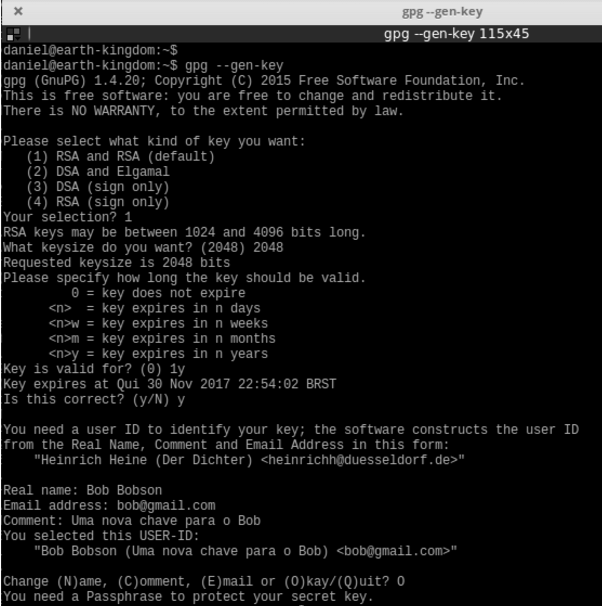
\includegraphics[width=0.9\textwidth]{./fig/1-gerar-chave.png}
 \caption{Comando e question�rio para gera��o de nova chave com GnuPG}
 \label{fig:exemploFig2}
\end{figure}


\begin{figure}[H]
 \centering
 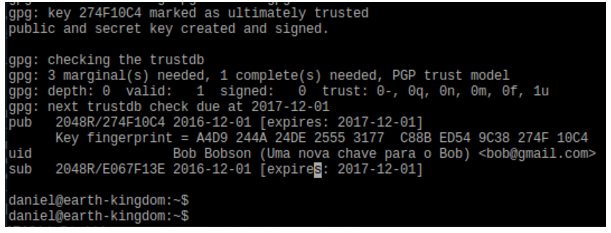
\includegraphics[width=0.9\textwidth]{./fig/gerar-chave-resutado.png}
 \caption{Resultado da gera��o da chave}
 \label{fig:exemploFig2}
\end{figure}


Para descriptografar a mesma mensagem usando a chave do usu�rio destinat�rio podemos usar o comando gpg --decrypt --output mensagem.original.txt  mensagem.cifrada.pgp

\begin{figure}[H]
 \centering
 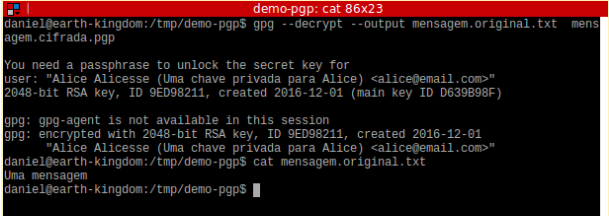
\includegraphics[width=0.9\textwidth]{./fig/3-decrypt-message.png}
 \caption{Resultado da gera��o da chave}
 \label{fig:exemploFig2}
\end{figure}